\documentclass{beamer}
\usepackage[utf8]{inputenc}
\usepackage[T2A]{fontenc}
\usepackage[english,russian]{babel}
\usepackage{graphicx} % Пакет для работы с изображениями
% \usepackage{tikz} % Required for creating the custom logo with opacity
\usepackage{adjustbox} % Hyperlinks

% \usetheme{default}
\definecolor{myblue}{RGB}{0,0,0} % Define black color (RGB values)
\setbeamercolor{frametitle}{fg=myblue} % Set frame title color to black
\setbeamerfont{frametitle}{series=\bfseries}
\setbeamertemplate{footline}[frame number]

\begin{document}

\begingroup
\setbeamertemplate{footline}{}
\begin{frame}
\begin{center}
    \begin{minipage}{0.1\textwidth}
        
\includegraphics[width=1.7cm]{img/bmstu_logo.jpg}
    \end{minipage}
    \hfill
    \begin{minipage}{0.80\textwidth}\centering
        {
            \linespread{1}\selectfont\tiny
            {Министерство науки и высшего образования~Российской~Федерации}

            {Федеральное~государственное~бюджетное~образовательное~учреждение высшего~образования}

            {<<Московский~государственный~технический~университет имени~Н.~Э.~Баумана (национальный~исследовательский~университет)>>}

            {(МГТУ им. Н.~Э.~Баумана)}
        }
    \end{minipage}
\end{center}
% \rule{\linewidth}{2.8pt}
\rule[3ex]{\linewidth}{1pt}

\begin{center}
    ПРЕЗЕНТАЦИЯ К КУРСОВОЙ РАБОТЕ НА ТЕМУ:
\end{center}

\vfill

\begin{center}
\textbf{Разработка программного обеспечения для моделирования упругих столкновений объектов в пространстве}
\end{center}

\vfill

Дисциплина: Компьютерная графика

Студент: Рунов Константин Алексеевич ИУ7-54Б

Научный руководитель: Павельев Александр Анатольевич

\vfill

\centering
Москва, 2023 г.
\end{frame}
\endgroup

% \logo{%
      % \begin{tikzpicture}[remember picture,overlay,opacity=0.5]
          % \node[anchor=north east] at (current page.north east) {
\includegraphics[width=4cm]{img/bmstu_logo.jpg}};
          % \node[anchor=north east] at (current page.north east) {\resizebox{5cm}{5cm}{\makebox[5cm][c]{
\includegraphics[width=3cm]{img/bmstu_logo.jpg}}}};
      % \end{tikzpicture}
% }

\begin{frame}
\frametitle{Цель}

Цель работы --- разработка программы для моделирования упругих столкновений объектов в пространстве.

\end{frame}
\begin{frame}
\frametitle{Задачи}
\begin{itemize}
    \item<1-> Описать свойства объекта, которыми он должен обладать для моделирования его движения и столкновения с другими объектами.
    % \item проанализировать существующие способы представления объектов;
    % \item проанализировать существующие алгоритмы обнаружения коллизий;
    % \item проанализировать существующие модели освещения;
    % \item<1-> Проанализировать существующие способы представления объектов, алгоритмы обнаружения коллизий и модели освещения и выбрать те из них, которые будут использованы при проектировании и разработке программы.
    \item<2-> Проанализировать существующие алгоритмы обнаружения коллизий и модели освещения и выбрать те из них, которые будут использованы при проектировании и разработке программы.
    \item<3-> На формальном языке описать выбранные алгоритмы, а также общие алгоритмы работы программы.
    \item<4-> Выбрать типы и структуры данных, которые будут использованы при разработке программы.
    \item<5-> Разработать программное обеспечение для решения поставленной задачи.
    \item<6-> Провести анализ зависимости времени генерации кадра от количества треугольников, их которых состоят модели объектов сцены; количества столкновений объектов сцены; количества вызовов функций графического ускорителя.
    % \item реализовать выбранные алгоритмы;
\end{itemize}
\end{frame}

\begin{frame}
\frametitle{Описание свойств объектов}
Для визуализации объекта, он должен содержать следующую информацию.
\begin{itemize}
    \item<1-> Геометрическая информация, какую форму имеет объект.
    \item<2-> Информация о местоположении в пространстве.
    \item<3-> Информация о цвете и/или текстуре объекта.
\end{itemize}
\end{frame}

\begin{frame}
\frametitle{Описание свойств объектов}
Для моделирования движения и столкновения объектов, объекты должны содержать следующую информацию.
\begin{itemize}
    \item<1-> Информация о <<коллайдере>>.
    \item<2-> Информация о физических свойствах объекта.
\end{itemize}

\end{frame}

\begin{frame}
\frametitle{Выбор алгоритмов обнаружения коллизий}
\begin{table}[H]
    \caption{Сравнение алгоритмов обнаружения коллизий}
    \label{tab:collisions}
\begin{adjustbox}{width=1\textwidth}
    \begin{tabular}{|p{.20\textwidth}|p{.20\textwidth}|p{.20\textwidth}|p{.20\textwidth}|p{.20\textwidth}|p{.20\textwidth}|}
        \hline
        &
        Алгоритм обнаружения коллизий сферы относительно сферы
        &
        Алгоритм AABB
        &
        Алгоритм OBB
        &
        Алгоритм GJK
        \\
        \hline
        Вычислитель-ная нагрузка
        &
        % Алгоритм обнаружения коллизий сферы относительно сферы
        1 % Низкая
        &
        % Алгоритм AABB
        1 % Низкая
        &
        % Алгоритм OBB
        2 % Средняя
        &
        % Алгоритм GJK
        3 % Высокая
        \\
        \hline
        Точность обнаружения коллизий у сложных объектов
        &
        % Алгоритм обнаружения коллизий сферы относительно сферы
        3 % Низкая
        &
        % Алгоритм AABB
        3 % Низкая
        &
        % Алгоритм OBB
        2 % Средняя
        &
        % Алгоритм GJK
        1 % Высокая
        \\
        \hline
        Сложность реализации
        &
        % Алгоритм обнаружения коллизий сферы относительно сферы
        1 % Низкая
        &
        % Алгоритм AABB
        1 % Низкая
        &
        % Алгоритм OBB
        2 % Средняя
        &
        % Алгоритм GJK
        3 % Высокая
        \\
        \hline
    \end{tabular}
\end{adjustbox}
\end{table}
Выбор: Алгоритм AABB
\end{frame}

\begin{frame}
\frametitle{Выбор модели освещения}

\begin{table}[H]
    \caption{Сравнение моделей освещения}
    \label{tab:lighting-models}
\begin{adjustbox}{width=1\textwidth}
    \begin{tabular}{|p{.20\textwidth}|p{.20\textwidth}|p{.20\textwidth}|p{.20\textwidth}|p{.20\textwidth}|}
        \hline
        &
        Простая модель освещения
        &
        Модель освещения Гуро
        &
        Модель Фонга
        \\
        \hline
        Реалистич-ность изображения
        &
        % Простая модель освещения
        3 % Низкая
        &
        % Модель освещения Гуро
        2 % Средняя
        &
        % Модель Фонга
        1 % Высокая
        \\
        \hline
        Вычислитель-ная нагрузка
        &
        % Простая модель освещения
        1 % Низкая
        &
        % Модель освещения Гуро
        2 % Средняя
        &
        % Модель Фонга
        3 % Высокая
        \\
        \hline
        Сложность реализации
        &
        % Простая модель освещения
        1 % Низкая
        &
        % Модель освещения Гуро
        2 % Средняя
        &
        % Модель Фонга
        2 % Средняя
        \\
        \hline
    \end{tabular}
\end{adjustbox}
\end{table}
Выбор: Модель Фонга
\end{frame}

\begin{frame}
\frametitle{Алгоритм AABB}
\centering
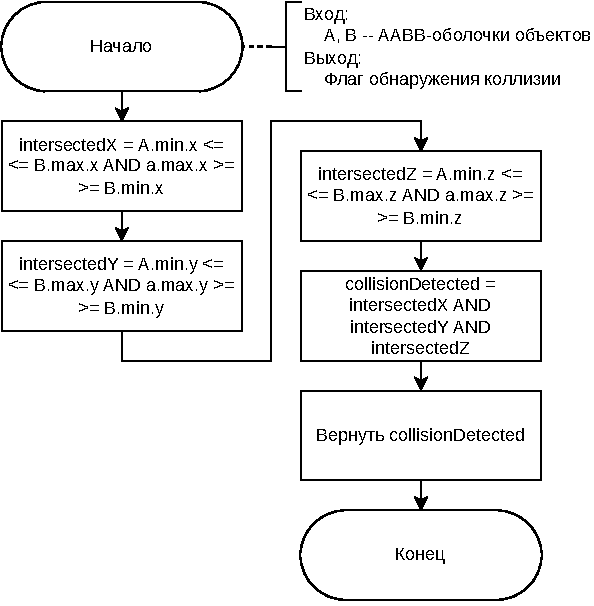
\includegraphics[scale=0.7]{diag/aabb_tighter.pdf}
\end{frame}

\begin{frame}
\frametitle{Модель Фонга}
В модели освещения Фонга учитываются три составляющих отражённого света:

    % \begin{minipage}{0.4\textwidth}
\begin{itemize}
    \item Рассеянная.
    \item Фоновая.
    \item Зеркальная.
\end{itemize}
% \end{minipage}
% \hfill
    % \begin{minipage}{0.5\textwidth}
\centering
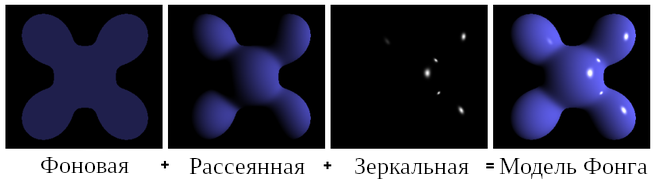
\includegraphics[width=1\textwidth]{img/phong-components}
% \end{minipage}
\end{frame}

\begin{frame}
\frametitle{Модель Фонга. Рассеянный свет}
\centering
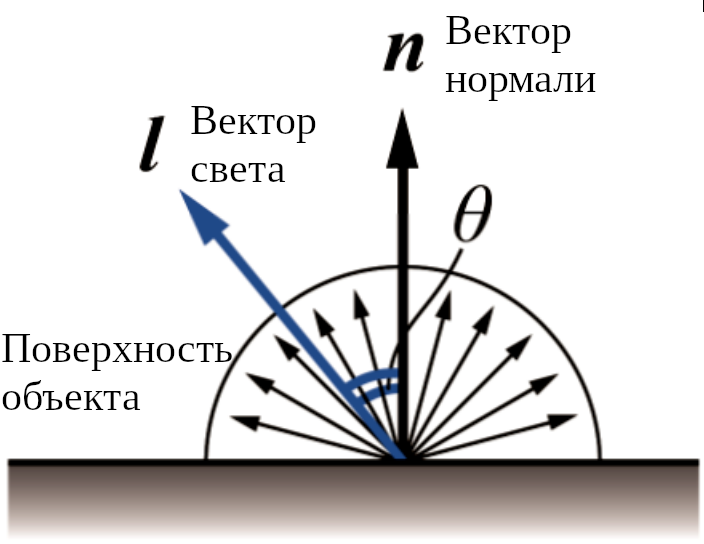
\includegraphics[width=0.56\textwidth]{img/diffuse_ru}
\begin{equation}
    I_d = k_d I_l \cos \theta = k_d I_l \left| \boldsymbol{n} \cdot \boldsymbol{l} \right|
    \label{eq:diffuse}
\end{equation}
\end{frame}

\begin{frame}
\frametitle{Модель Фонга. Фоновое освещение}
\centering
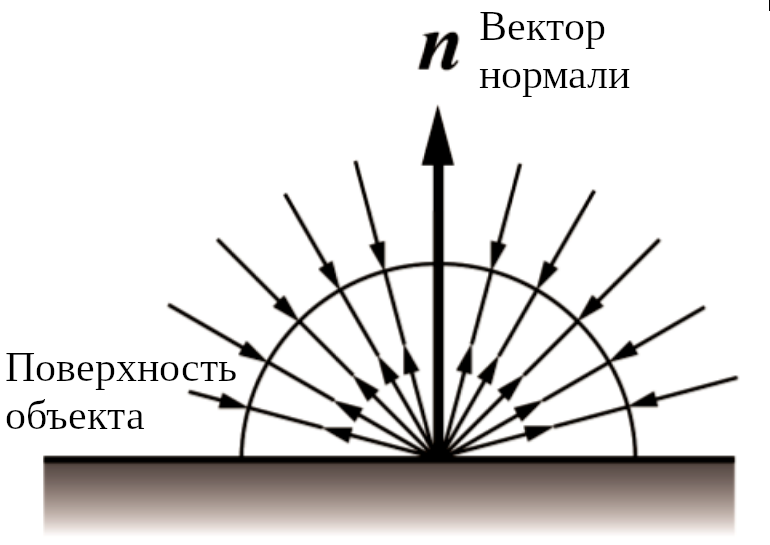
\includegraphics[width=0.6\textwidth]{img/ambient_ru}
\begin{equation}
    I_a = k_a I_0
    \label{eq:ambient}
\end{equation}
\end{frame}

\begin{frame}
\frametitle{Модель Фонга. Зеркальный свет}
\centering
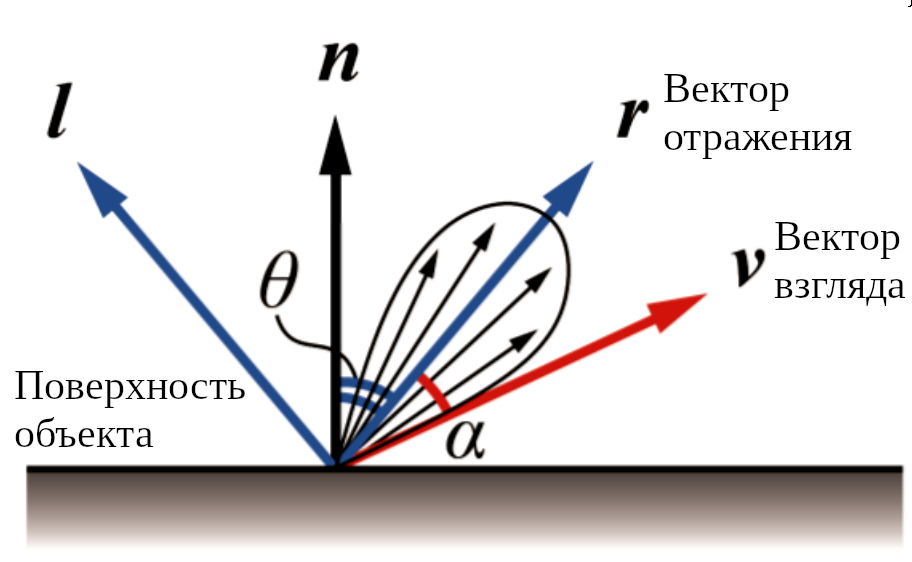
\includegraphics[width=0.66\textwidth]{img/specular_ru}
\begin{equation}
    I_s = k_s I_l \cos^n \alpha = k_s I_l \left| \boldsymbol{r} \cdot \boldsymbol{v} \right|^n
    \label{eq:specular}
\end{equation}
\end{frame}

\begin{frame}
\frametitle{Общий алгоритм работы программы}
\centering
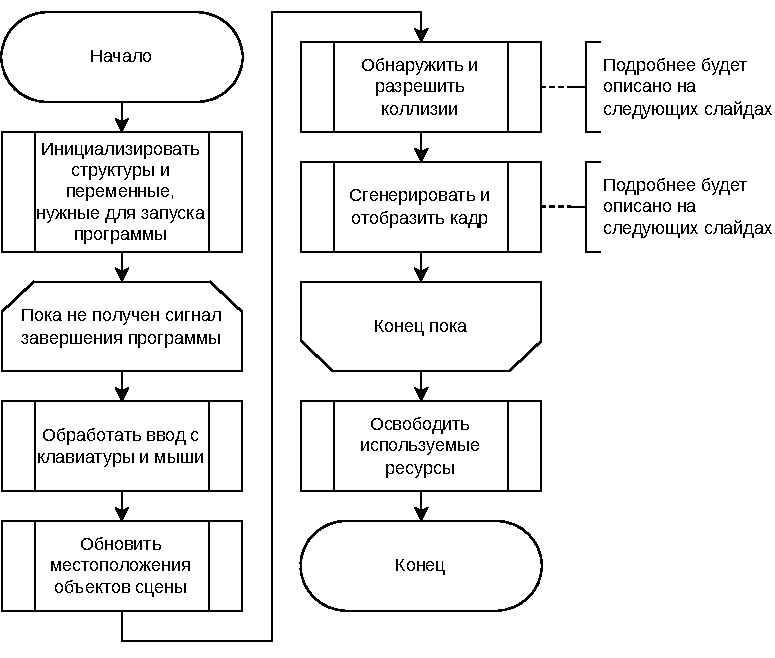
\includegraphics[scale=0.75]{diag/common-algo-for-pres.pdf}
\end{frame}

\begin{frame}
\frametitle{Общий алгоритм обнаружения и разрешения коллизий}
\centering
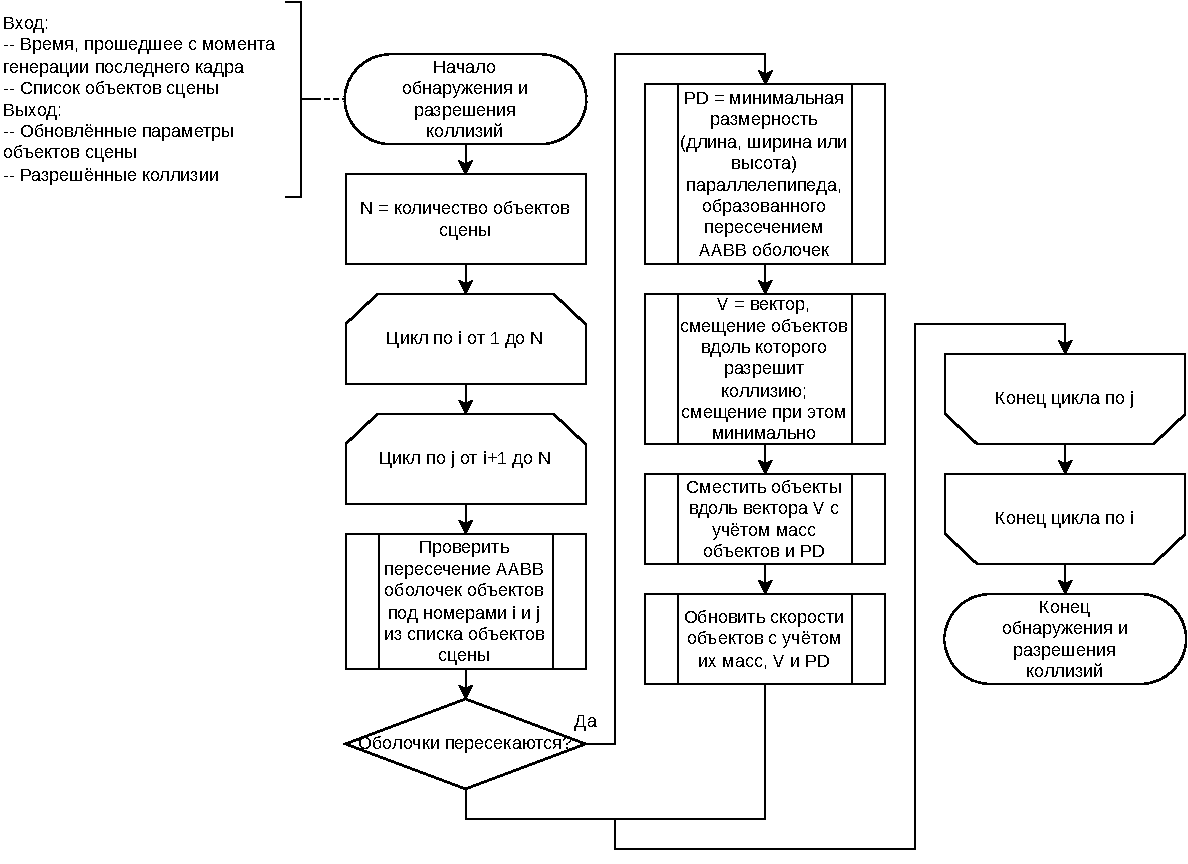
\includegraphics[scale=0.55]{diag/collisions-algo.pdf}
\end{frame}

\begin{frame}
\frametitle{Общий алгоритм генерации и отображения кадра}
\centering
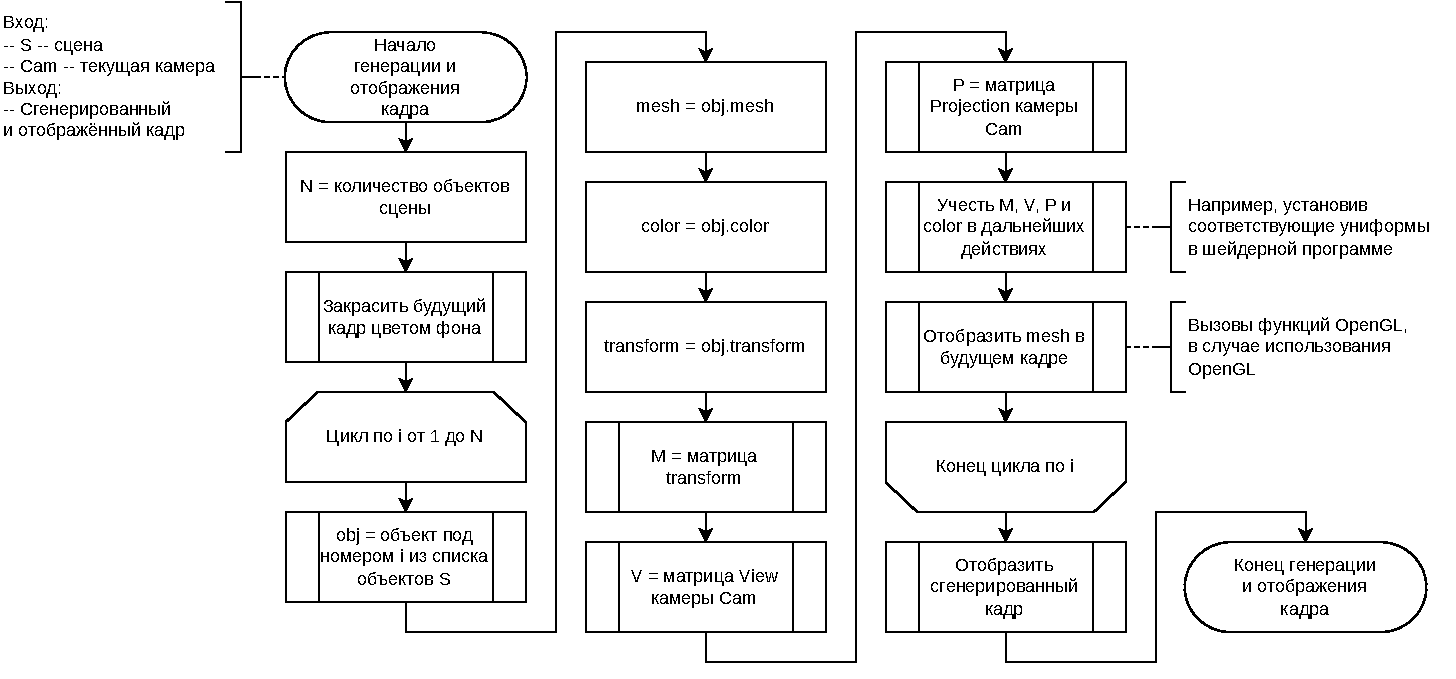
\includegraphics[scale=0.48]{diag/frame-gen-algo.pdf}
\end{frame}

\end{document}
